\documentclass[12pt]{article}%
\usepackage{amsmath,amssymb,amsthm,amsfonts}
\usepackage{wasysym}
\usepackage{graphicx}
\usepackage[dvipsnames]{xcolor}
\usepackage{stackengine}
\def\stackalignment{l}
\usepackage[colorlinks]{hyperref}
\usepackage{tikz}
\usepackage[export]{adjustbox}

\ProvidesPackage{commands}

%---Packages---%
\usepackage{amssymb, fullpage, amsmath, esint}
\usepackage{graphicx}
\usepackage{empheq}
\usepackage{float}
\usepackage{listings}
\usepackage{color}
\usepackage{caption}
\usepackage{subcaption}


%---Environments---%
\newtheorem{problem}{Problem}
\newenvironment{solution}[1][\it{Solution}]{\textbf{#1. } }{$\square$}

%---Style---%
\graphicspath{ {./} }
\allowdisplaybreaks
\pagestyle{empty}
%\numberwithin{equation}{subsection}


%---Definitions---%
\def\Z{{\mathbb Z}}
\def\Q{{\mathbb Q}}
\def\C{{\mathbb C}}
\def\R{{\mathbb R}}
\def\N{{\mathbb N}}
\def\eps{{\epsilon}}
\def\O{{\mathcal{O}}}
\def\F{{\mathcal{F}}}
\def\ointcc{{\ointctrclockwise}} %counter clockwise contour integral
\def\ointc{{\ointclockwise}} %clockwise contour integral
\def\and{{~\text{and}~}} %and


%dash integral 
\def\Xint#1{\mathchoice
   {\XXint\displaystyle\textstyle{#1}}%
   {\XXint\textstyle\scriptstyle{#1}}%
   {\XXint\scriptstyle\scriptscriptstyle{#1}}%
   {\XXint\scriptscriptstyle\scriptscriptstyle{#1}}%
   \!\int}
\def\XXint#1#2#3{{\setbox0=\hbox{$#1{#2#3}{\int}$}
     \vcenter{\hbox{$#2#3$}}\kern-.5\wd0}}
\def\ddashint{\Xint=}
\def\dashint{\Xint-}


%---Commands---%
\newcommand{\floor}[1]{{\left\lfloor#1\right\rfloor}} % Floor function
\newcommand{\ceil}[1]{{\left\lceil#1\right\rceil}} % Ceiling function
\newcommand{\paren}[1]{{\left(#1\right)}} % Parentheses ()
\newcommand{\brac}[1]{{\left\{#1\right\}}} % Curly braces {}
\newcommand{\braces}[1]{{\left[#1\right]}} % Braces []
\newcommand{\abrac}[1]{{\left\langle#1\right\rangle}} % Angle Braces <>
\newcommand{\abs}[1]{{\left|#1\right|}} % Absolute value
\newcommand{\norm}[1]{{\left\|#1\right\|}} % Norm
\newcommand{\eval}[2]{\right|_{#1}^{#2}} % Evaluate
\newcommand{\pp}[2]{\frac{\partial #1}{\partial #2}} % Partial of 1 wrt 2
\newcommand{\ppn}[3]{\frac{\partial^{#1} #2}{\partial #3^{#1}}} % nth Partial of 1 wrt 2
\newcommand{\dd}[2]{\frac{\mathrm{d} #1}{\mathrm{d} #2}} % Partial of 1 wrt 2
\newcommand{\ddn}[3]{\frac{\mathrm{d}^{#1} #2}{\mathrm{d} #3^{#1}}} % nth Partial of 1 wrt 2
\newcommand\fullref[1]{Eq.~(\ref*{#1})} % Eq.()
\newcommand\dt[1]{\mathrm{d}#1} %dt

%boxed solution with spacing 0.5cm around equations
\setlength\fboxsep{0.5cm}
\newcommand*\widefbox[1]{\fbox{#1}}


%MATLAB formatting
\definecolor{mygreen}{rgb}{0,0.6,0}
\definecolor{mygreen}{RGB}{28,172,0} % color values Red, Green, Blue
\definecolor{mylilas}{RGB}{170,55,241}
\definecolor{light-gray}{gray}{0.95} %the shade of grey that stack exchange uses
\lstset{ 
    backgroundcolor=\color{light-gray},
}
\lstset{language=Matlab,%
    %basicstyle=\color{red},
    breaklines=true,%
    morekeywords={matlab2tikz},
    keywordstyle=\color{blue},%
    morekeywords=[2]{1}, keywordstyle=[2]{\color{black}},
    identifierstyle=\color{black},%
    stringstyle=\color{mylilas},
    commentstyle=\color{mygreen},%
    showstringspaces=false,%without this there will be a symbol in the places where there is a space
    numbers=left,%
    numberstyle={\tiny \color{black}},% size of the numbers
    numbersep=9pt, % this defines how far the numbers are from the text
    emph=[1]{for,end,break},emphstyle=[1]\color{red}, %some words to emphasise
    %emph=[2]{word1,word2}, emphstyle=[2]{style},    
}


%\usepackage{geometry}
%\geometry{top = 0.9in}
\usepackage{appendix}

\numberwithin{equation}{subsection}

\renewcommand{\S}{\mathbb{S}^1}
\renewcommand{\Re}{\text{Re}}
\newcommand{\ea}{\textit{et al. }}
\renewcommand{\epsilon}{\varepsilon}
\renewcommand{\th}{\text{th}}
\newcommand{\sgn}{\operatorname{sgn}}

\renewcommand{\setminus}{\smallsetminus}

\newtheorem{thm}{Theorem}
\newtheorem{lemma}{Lemma}

\definecolor{red}{rgb}{0.8500, 0.3250, 0.0980}
\definecolor{green}{rgb}{0.4660, 0.6740, 0.1880}
\definecolor{yellow}{rgb}{0.9290, 0.6940, 0.1250}
\definecolor{blue}{rgb}{0, 0.4470, 0.7410}


\begin{document}

\title{Coding Project 4:  Teaching a Computer to Recognize Written Numbers}

\author{Marvyn Bailly}
\date{}

\maketitle


\begin{abstract}
In this coding project, we begin with a brief history and applications of machine learning. We continue to discuss the elements of the mathematical theory behind Linear Discriminant Analysis which include the Rayleigh quotient, SVD, and wavelet basis. Next we create an image recognition program using the concepts of Linear Discriminant Analysis to classify images of handwritten ones and zeros. We continue to extend the program using a "one vs all" method to recognize numbers zero through nine. Lastly we test the success rate of the program on a self-created dataset of handwritten numbers. Before concluding, we summarize the report and discuss the effectiveness of the LDA method at image recognition.  
\end{abstract}


\section{Introduction}
\label{Sec: Intro}


As artificial intelligence driven projects such as ChatGBT and Bing's search engine take the internet by storm, it is important to understand the basics of how machine learning works. ML is a powerful and rapidly evolving field in computer science that enables a program to learn from training data, without being explicitly programmed to preform a task. In other words, it is a way for machines to improve their performance on a task without human intervention. Machine learning is driven by algorithms that can detect patterns and make predictions based on the initial training data they are given and improve upon themselves by learning from its mistakes. With the increasing availability of large data, advances in computing power and learning algorithms, machine learning is now used in a wide range of applications, from speech recognition, to chatbots, to fraud detection systems. The uses of machine learning promises to revolutionize the way we live, work, and interact with technology.  

\bigskip
\bigskip

In this report, we will examine a classic example of machine learning by training a program to recognize hand written numbers through dimensionality reduction and Linear Discriminant Analysis. We will begin by explaining the mathematical theoretical background behind Linear Discriminant Analysis and how it can be applied to datasets to find colorations and differences within and between datasets. Next we will present the results of applying the concepts in MATLAB on a subset of Yann LeCun's famous data set of written numbers to create a program that can recognize the difference between the numbers 0 and 1. We will continue to extend the program to identify numbers 0 to 9 and test the effectiveness using a data set of numbers in addition to our own handwritten numbers. Finally, we will conclude the report with a discussion on the effectiveness of the presented method of image recognition.



\section{Theoretical Background}

In this section, we will discuss the mathematical theory of Linear Discriminant Analysis (LDA) and how it can be used in combination with the SVD and wavelet basis to classify images. 


\subsection{Linear Discriminant Analysis}

To understand how LDA works, we begin with two datasets of images. In our case, we will use a dataset containing images of handwritten zeros and another of ones. To correctly set up the data for LDA, we first concatenate the two datasets and apply a wavelet transform on them. Next we will preform a low rank approximation on the transformed dataset using the Singular Value Decomposition (SVD) and studying the singular values to determine the required degree for the rank approximation. Now that we have appropriately set up the data, we are ready to preform LDA on it.

The goal of LDA is to find the best projection that clusters data corresponding to the same set while separating data from different sets. In other words, we wish to maximize the distance between the inter-class data while minimizing the intra-class data. In our case, we are using two-class LDA as we have two datasets corresponding to zeros and ones, note that we re-separate the datasets after applying the wavelet transform and taking a rank-n approximation. To achieve the goal of LDA, we will construct a projection $\mathbf{w}$ using the generalized Rayleigh quotient of the form
\begin{equation} \label{rq}
    \mathbf{w} = \arg \max_{\mathbf{w}} \frac{\mathbf{w}^T \mathbf{S}_B \mathbf{w}}{\mathbf{w}^T \mathbf{S}_W \mathbf{w}},
\end{equation}   
where the scatter matrices for between-class, $\mathbf{S}_B$, and within-class, $\mathbf{S}_W$, are given by
\begin{equation}
    \mathbf{S}_B = (\mu_2 - \mu_1)(\mu_2 - \mu_1)^T,
\end{equation}
\begin{equation}
    \mathbf{S}_W = \sum_{j = 1}^{2} \sum_{\mathbf{x}} (\mathbf{x} - \mu_j)(\mathbf{x} - \mu_j)^T,
\end{equation}
where $\mu_i$ corresponds to the mean of the $i^{\text{th}}$ dataset. Then we look at the solution to generalized Rayleigh quotient \fullref{rq} which can be found by studying the corresponding eigenvalue problem of the form
\begin{equation}
    \mathbf{S}_B \mathbf{w} = \lambda \mathbf{S}_W \mathbf{w},
\end{equation}
where the maximum eigenvalue $\lambda$ and its corresponding eigenvector form the desired projection basis for the dataset. Now that we have constructed a projection that appropriately separates the data, we can compute a threshold value between the datasets. In our case, we compute a threshold value that separates images corresponding to ones from those that correspond to zeros. This allows us to pass in new images and classify their type using the threshold value found using the LDA method.  


\section{Results}

\begin{figure}
    \begin{subfigure}[b]{0.5\linewidth}
        \centering
        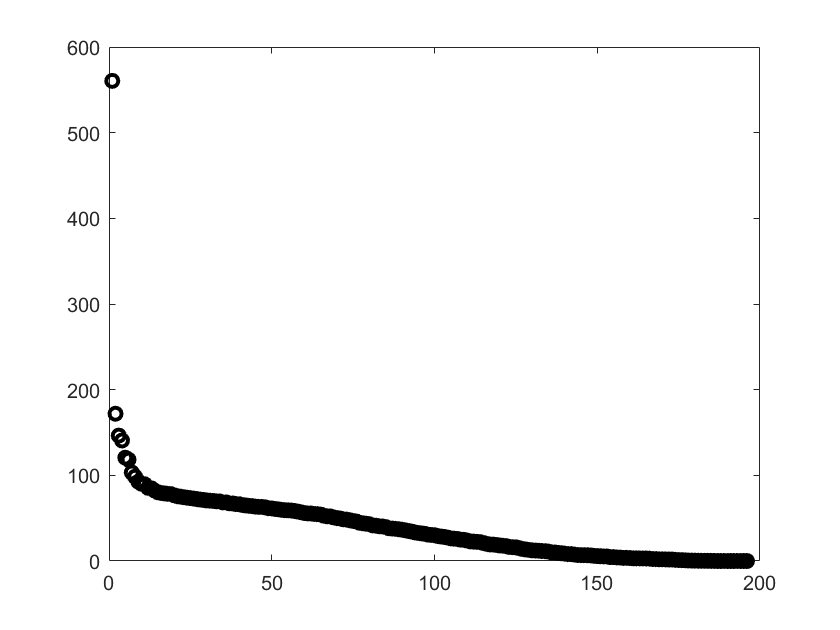
\includegraphics[width=\linewidth]{images/1a.png}
        \caption{Plot of Singular Values.}
        \label{fig1:a}
        \vspace{4ex}
    \end{subfigure}%%
    \begin{subfigure}[b]{0.5\linewidth}
        \centering
        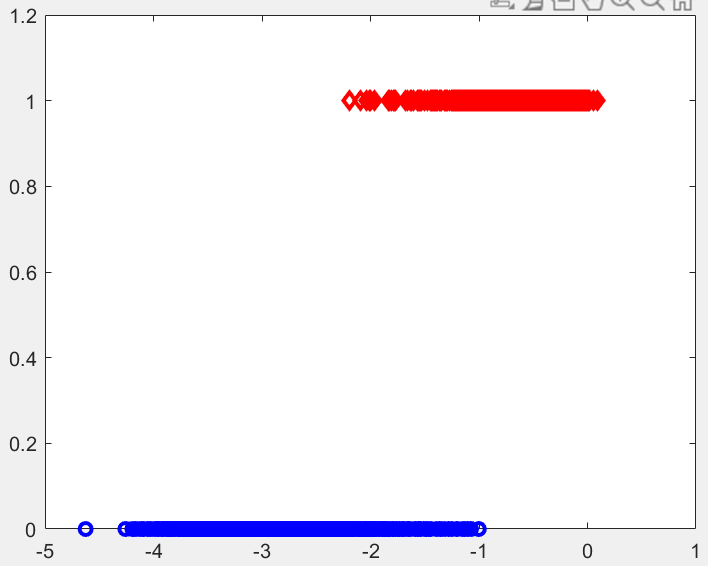
\includegraphics[width=\linewidth]{images/2a.PNG}
        \caption{Plot of projected data using LDA.}
        \label{fig1:b}
        \vspace{4ex}
    \end{subfigure}
    \caption{In figure (a) we see a plot of the singular values of the concatenated datasets corresponding to zeros and ones. In figure (b) we see data points corresponding to zeros in blue and the data points corresponding to ones in red in the projected space found using LDA. To demonstrate how the project separates the data, we plot zeros along $y=0$ and ones along $y=1$. }
    \label{fig1}
\end{figure}


To apply the LDA method on Yann LeCun's dataset, we will take a subset of the dataset corresponding to handwritten ones and zeros. We will begin by setting up the data as described in Section (2.1). To find an appropriate rank-n approximation of the dataset, we study the singular values from the SVD of dataset. The singular values can be seen in Figure 1(a) where we determined that the first $15$ singular values and their corresponding components should be used to approximate the dataset. This allows us to work with a smaller dataset that maintains the important characteristics of the original datasets. We continue to apply the LDA method to find a projector that projects the data into separated sets. In Figure 1(b) we see the result of applying the projector to the ones and zeros dataset. To demonstrate the separating effect, the zeros are plotted in blue along $y=0$ and the ones are plotted in red along $y=1$. We see that the two datasets are separated and the points within the same dataset are clustered as desired. Now we can use the eigenvalue problem to find the threshold value between the two datasets to be $-1.5541$. 

Now that we have found the threshold value between the two sets, we can give the program a dataset that contains both zeros and ones randomly distributed. Applying the same set up and LDA method to the test data, we can classify the data points within the test data set into ones and zeros using the threshold value that we found. Comparing the results of program with the actual classes of the data, we see that the program can effectively identify the zeros and ones with a $99.72 \%$ success rate. Now that we are able to identify the difference between zeros and ones, we wish to extend the program to identify numbers zero to nine. Up until now, we have been using a "one vs. another" method to apply the two-class LDA method to the datasets. To modify our approach to train the program on multiple numbers but still use a two-class approach, we will use a "one vs. all" approach.

In the "one vs. all" approach, we use the LDA method to find a threshold value between the desired number and all other numbers. To do this, we repeat the same process as outline for ones and zeros but now place the desired number in one dataset and all other numbers in the second data set. For example, if we want to train the program to identify zero, all the data points corresponding to zero are place in one set while the rest of the numbers, one through nine, are placed in the other. Repeating this process for all numbers, we come up with threshold values for each number compared to all other numbers. In Figure 2 and 3, we can see the projections of each numbers compared to all other numbers and observe that the method once again is able to separate the different sets while clustering points within the same set. Now that we have found the thresholds, we can test the program against a random test set of numbers and compute the accuracy of our program. The results are summarized in Table 1 where we see the classification success rate of each number. The program achieved its highest success rate of $95.35\%$ using the "one vs. all" method when classifying $1$ and its lowest success rate of $77.10\%$ while classifying $5$. 

Finally we tested the program with a dataset that we created ourselves. To do this, we hand wrote the numbers zero to nine and passed them to the program. In Table 1, we see on the right column that the handwritten examples had a low success rate with only 1,4,5, and 7 being detected consistently throughout different attempts of handwritten numbers. Thus we see that the success rate of the program applied to a dataset that differs from the set used to train upon is significantly lower.

\begin{table}
    \centering
    \begin{tabular}{ccc}
          Number of Interest &   Success Rate &   Personal Handwritten Number\\
        \hline\hline
         0 &  90.12\% &  No\\
       
         1 &  95.35\% &   Yes\\
       
         2 &  84.93\% &   No\\
       
         3 &  81.64\% &   No\\
       
         4 &  82.02\% &   Yes\\
       
         5 &  77.10\% &   Yes\\
       
         6 &  90.83\% &  No\\
       
         7 &  91.86\% &  Yes\\
       
         8 &  82.54\% &  No\\
       
         9 &  86.43\% &  Yes\\
    \end{tabular}
    \caption{The success rate of each number trained against all others applied to the test data set. The last columns shows if the program was able to identify our own handwritten numbers consistently over a series of few attempts.}
    \label{Table}
\end{table}
\normalsize





\section{Conclusion}\label{Sec: Conclusion}
In summary, for this coding project, we briefly discussed the applications and history of machine learning. Next we motivated the use of LDA in image recognition before describing the theoretical background behind LDA in combination with the SVD and wavelet transform. We continued to outline the process of setting up and applying LDA in an image recognition program. We presented the results of the program when trained on a dataset containing images of handwritten ones and zeros. We continued to extend the program to detect numbers zero through nine and achieved a reasonable success rates when testing the program on the test dataset. Finally we applied the program on our own handwritten numbers which yielded a significantly lower success rate. 

While we were able to achieve a higher success rate than $77\%$ on all the numbers, we didn't change the method to compute the thresholds. We applied the same "one vs. another" process as seen in the case for ones and zeros dataset but instead of "another" used "all." We only slightly modified the success rate computation to extend to higher dimensions. We also made a note that the program was less success with datasets different from that it was trained upon. We believe that this is a result of the method we used. Our leading theories on why this is the case is that either the "one vs all" method didn't translate well over to two-class LDA method or that the LDA method has a lower success rate than other image recognition processes. It would be interesting to test higher class LDA methods (if this is a thing?) and check their success rate on different data sets. It would also be interesting to try other methods of image recognition and compare the results. 

\section*{Acknowledgment}

I would like to acknowledge the help I received from Kaitlynn Lily and Alex Johnson. Kaitlynn provided help with the created the "one vs. all" method and Alex helped me rewrite my code in Python so that I could generated the plots. For some reason my laptop was unable to create the plots in MATLAB as MATLAB would either crash, create inconsistent graphs, or run out of memory while trying to generate the graphs. 

\begin{figure}[H]
    \begin{subfigure}[b]{0.5\linewidth}
        \centering
        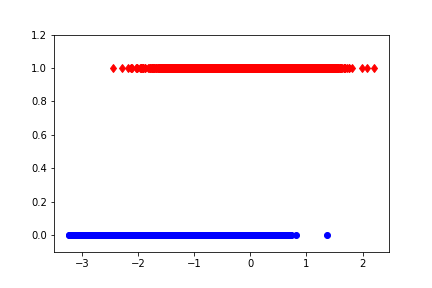
\includegraphics[width=\linewidth]{images/fig0.png}
        \caption{Plot of projected data in zero vs all.}
        \label{fig2:a}
        \vspace{4ex}
    \end{subfigure}%%
    \begin{subfigure}[b]{0.5\linewidth}
        \centering
        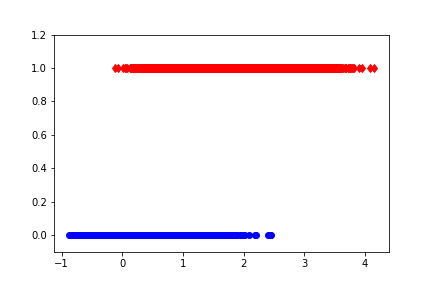
\includegraphics[width=\linewidth]{images/fig1.png}
        \caption{Plot of projected data in one vs all.}
        \label{fig2:a}
        \vspace{4ex}
    \end{subfigure}%%
    


    \begin{subfigure}[b]{0.5\linewidth}
        \centering
        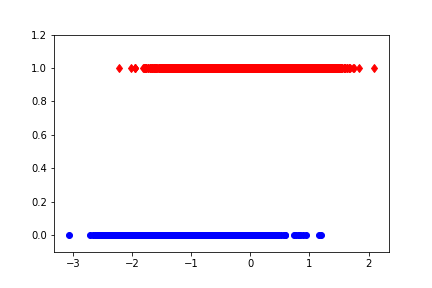
\includegraphics[width=\linewidth]{images/fig2.png}
        \caption{Plot of projected data in two vs all.}
        \label{fig2:a}
        \vspace{4ex}
    \end{subfigure}%%
    \begin{subfigure}[b]{0.5\linewidth}
        \centering
        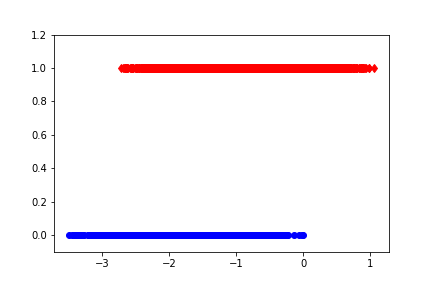
\includegraphics[width=\linewidth]{images/fig3.png}
        \caption{Plot of projected data in three vs all.}
        \label{fig2:a}
        \vspace{4ex}
    \end{subfigure}%%
    
    
    
    \begin{subfigure}[b]{0.5\linewidth}
        \centering
        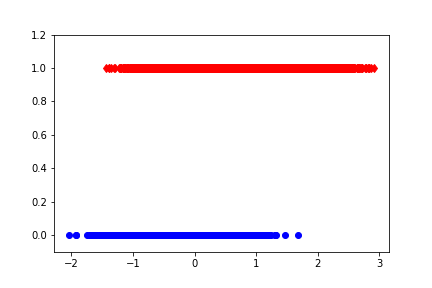
\includegraphics[width=\linewidth]{images/fig4.png}
        \caption{Plot of projected data in four vs all.}
        \label{fig2:a}
        \vspace{4ex}
    \end{subfigure}%%
    \begin{subfigure}[b]{0.5\linewidth}
        \centering
        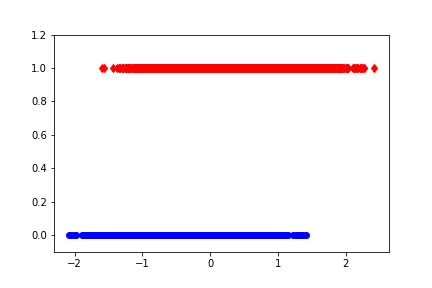
\includegraphics[width=\linewidth]{images/fig5.png}
        \caption{Plot of projected data in five vs all.}
        \label{fig2:a}
        \vspace{4ex}
    \end{subfigure}%%

        \caption{Plots of data points corresponding to the number of interest vs all other numbers projected onto the basis found via LDA. To demonstrate the separating and clustering effect of the method, the data points corresponding to the number of interested are plotted along $y=0$ while all others along $y=1$.}
    \label{fig2}
\end{figure}

\begin{figure}[H]
    \begin{subfigure}[b]{0.5\linewidth}
        \centering
        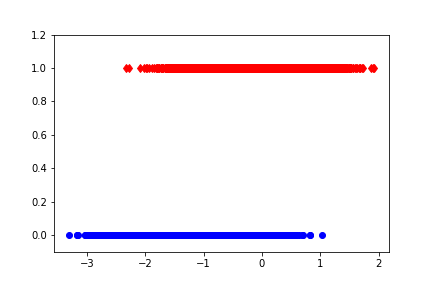
\includegraphics[width=\linewidth]{images/fig6.png}
        \caption{Plot of projected data in six vs all.}
        \label{fig3:a}
        \vspace{4ex}
    \end{subfigure}%%
    \begin{subfigure}[b]{0.5\linewidth}
        \centering
        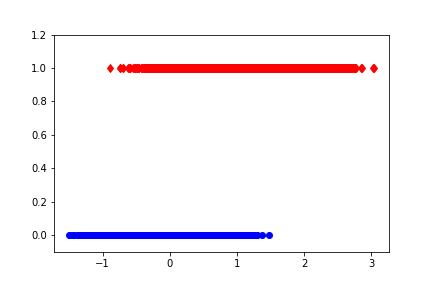
\includegraphics[width=\linewidth]{images/fig7.png}
        \caption{Plot of projected data in seven vs all.}
        \label{fig3:b}
        \vspace{4ex}
    \end{subfigure}


    \begin{subfigure}[b]{0.5\linewidth}
        \centering
        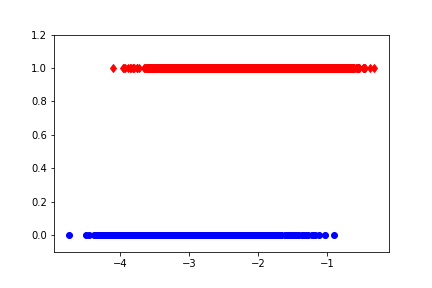
\includegraphics[width=\linewidth]{images/fig8.png}
        \caption{Plot of projected data in eight vs all.}
        \label{fig3:a}
        \vspace{4ex}
    \end{subfigure}%%
    \begin{subfigure}[b]{0.5\linewidth}
        \centering
        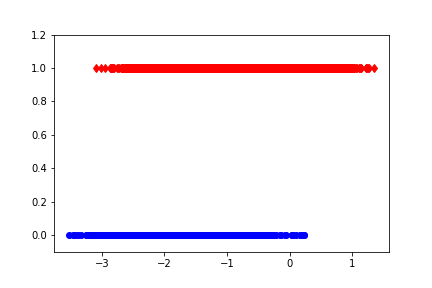
\includegraphics[width=\linewidth]{images/fig9.png}
        \caption{Plot of projected data in nine vs all.}
        \label{fig3:b}
        \vspace{4ex}
    \end{subfigure}
    \caption{Plots of data points corresponding to the number of interest vs all other numbers projected onto the basis found via LDA. To demonstrate the separating and clustering effect of the method, the data points corresponding to the number of interested are plotted along $y=0$ while all others along $y=1$.}
    \label{fig3}
\end{figure}

\end{document}
